\section*{Dati e risultati}

\subsection*{Termometro elettrico}

In questa sezione vogliamo illustrare come abbiamo realizzato e lo scopo del circuito illustrato in Figura \ref{fig:termometro}. Quindi andremo a spiegarne il funzionamento genrale, dei singoli blocchi e i ragionamenti fatti al fine di realizzarlo.
Come già anticipato questo circuito ha lo scopo di misurare la temperatura di un ambiente in base al valore di resistenza assunto dal trasduttore di temperature Pt100 o temoresistenza Pt100 (questi due termini verranno usati indistintamente) fornendo allo sperimentatore una misura di differenza di potenziale facilmente convertibile in $^\circ$C.

Quindi come prima cosa suddividiamo il circuito in Figura \ref{termometro} in quattro blocchi fondamentali.
Il primo è costituito dal circuito integrato REF02, che è un generatore di tensione di riferimento $\SI{+5}{\volt}$ costante.
Il secondo blocco è costituito dall'amplificatore operazionale OP07 e dalla termoresistenza Pt100.
Il terzo blocco è formato dal secondo amplificatore operazionale OP07.
Infine il quarto ed ultimo blocco del circuito è costituito dall'amplificatore per strumentazione AD622.

Detto questo andiamo ad analizzare singolarmente i quattro blocchi:

\paragraph*{$1^\circ$ Stadio:}

Questo è formato dal circuito integrato REF02, che molto semplicemente ha la funzione di fornire in ingresso al nostro circuito una tensione costante di $\SI{+5}{\volt}$ che non presenta variazioni significative fino all'ordine dei $\si{\milli\volt}$, che abbiamo verificato direttamente.
Come è possibile notare questo circuto è stato alimentato con una tensione costante di $\SI{+15}{\volt}$ fornita dal generatore di tensione costante.

\paragraph*{$2^\circ$ Stadio:}

Questo è composto dall'amplificatore operazionale OP07, la termoresistenza Pt100 e le resistenze di feedback. Questo blocco è una sorgente di corrente costante. Infatti uno degli obbiettivi è quelo di fornire al trasduttore di temperature Pt100 una corrente costante dell'ordine di $\SI{1}{\milli\ampere}$ al fine di evitare effetti di autoriscaldamento, per effetto Joule, che potrebbero compromettere la bontà della misura di resistenza. Quindi $I\ped{Pt100}\,=\,\SI{1}{\milli\ampere}$. Quindi, grazie alla configurazione di amplificatore invertente, possimo determinare il valore di resistenza che deve essere applicato all'ingresso invertente al fine difar scorrre una corrente di $\SI{1}{\milli\ampere}$ nel ramo di retroazione negativo e quindi nella termoresistenza. Grazie alle regole per amplificatori operazionali e alla legge di Ohm otteniamo che:
\begin{equation}
	R\,=\,\frac{V\ped{in1}}{I\ped{Pt100}}\,=\,\SI{5}{\kilo\ohm}
\end{equation}
dove con $V\ped{in1}$ indichiamo la tensione in ingresso all'amplificatore e con $R$ il valore di resistenza che deve essere usato all'ingresso invertente.
Quindi con questi valori sappiamo anche che a $0\,^\circ$C la tensione in uscita dall'amplificatore $V\ped{out1}$ ha un valore di $\SI{100}{\milli\volt}$ e che per ogni $^\circ$C la differenza di ptenziale in uscita $\Delta V\ped{out1}$ varia di $0.385\,\frac{\si{\milli\volt}}{^\circ C}$ poichè la variazione di resistenza ogni $^\circ$C vale $\Delta R\ped{Pt100}\,=\,0.385\,\frac{\si{ohm}}{^\circ C}$.

Osserviamo inoltre che la potenza dissipata $W$ per effetto Joule sulla termoresistenza ogni variazione positiva di $1^\circ$C può essere facilmente ricavata in quanto: 
\begin{equation}
	W\,=\,\Delta V\ped{in1} \cdot I\ped{Pt100}\,=\,10^{-4}\,\si{\watt}
\end{equation}

\paragraph*{$3^\circ$ Stadio:}

Anche in questo caso abbiamo come nucleo del blocco un amplificatore operazionale OP07. Tuttavia in questo caso il suo compito è quello di amplificare la tensione all'ingresso invertente $V\ped{in2}\,\equiv\,V\ped{out1}$. Ora per analizzare questo blocco è necessario anticipare parte delle considerazioni relative al $4^\circ$ stadio. Infatti noi vogliamo che in uscita da questo blocco $V\ped{out2}$ vi sia una differenza di potenziale di $\SI{5}{\volt}$ in modo tale che quando la temperaura è a $0\,^\circ$C $R\ped{Pt100}\,=\,\SI{100}{\ohm}$ e in uscita dall'amplificatore per strumentazione si legga una differenza di potenziale nulla, visto che i due ingressi sono alla stessa tensione.
Quindi al fine di realizzare questo proposito possiamodeterminare il guadagno che deve avere l'amlificatore operazionale OP07, infatti:
\begin{equation}
	G_3\,=\,\frac{V\ped{out2}}{V\ped{in2}}\,=\,\frac{\SI{5}{\volt}}{\SI{0.1}{\volt}}\,=\, 50
	\qquad \text{e sapendo che} \qquad
	G_3\,=\,\frac{R_2}{R_1}
	\label{eq:G3}
\end{equation}
fissando arbitrariamente $R_2\,=\,\SI{100}{\kilo\ohm}$ otteniamo che $R_1\,=\,\SI{2}{\kilo\ohm}$.

\paragraph*{$4^\circ$ Stadio:}

Questo blocco è incentrato soprattutto sull'amplificatore differenziale per strumentazione AD622. Come già anticipato in precedenza vogliamo che quando la termoresistenza Pt100 vale $\SI{100}{\ohm}$ e quindi la temperature dell'ambiente è di $0\,^\circ$ in output $V\ped{out3}$ si legga un valore di tensione nullo.
Inoltre noi vogliamo che per ogni variazione del segnale in ingresso $V\ped{in2}$ di $\SI{0.385}{\milli\volt}$ in uscita $V\ped{out3}$ abbia un valore di $\SI{100}{\milli\volt}$. In questo modo la lettura diretta della differenza di potenziale $V\ped{out3}$ può fornire immediatamente un corrispettivo valore di temperatura semplicemente moltiplicando per dieci il valore di tensione che viene letto. Infatti si avrebbe che per ogni $^\circ$C la tensione $V\ped{out3}$ varia di $\SI{0.1}{\volt}$.

Quindi come prima cosa andiamo a valutare il guadagno complessivo che dobbiamo avere tra il $3^\circ$ e il $4^\circ$ stadio. Il guadagno totale $G$ corrisponde al rapporto tra $\frac{V\ped{out3}}{V\ped{in2}}$, quindi:
\begin{equation}
	G\,=\,\frac{\SI{100}{\milli\volt}}{\SI{0.385}{\milli\volt}}\,\simeq\,259.7
\end{equation}
Tuttavia sappiamo anche che $G\,=\,G_3 \cdot G_4$ e ricordandoci che $G_3\,=\,50$ grazie all'equazione (\ref{eq:G3}) possiamo ottenere che:
\begin{equation}
	G_4\,=\,\frac{G}{G_3}\,=\,5.19
\end{equation}

Ora che abbiamo trovato quanto deve valere il guadagno dell'amplificatore per strumentazione ($G_4$) possiamo determinare il valore della resistenza $R\ped{gain}$ che ci permette di ottenere il risultato desiderato. Noi sappiamo che:
\begin{equation}
	R\ped{gain}\,=\,\frac{\SI{50.5}{\kilo\ohm}}{G_4 - 1}\,\simeq\,\SI{12.05}{\kilo\ohm}
	\label{eq:Rgain}
\end{equation}


Con questo abbiamo finito di discutere i componenti del circuito e le loro funzioni. Tuttavia vogliamo precisare che per avere dei valori di tensione in uscita dai vari blocchi, che fossero quelli desiderati, le resistnze di ugni blocco sono state realizzate con una serie tra una resistenza prossima al valore stabilito e una resistenza variabile (trimmer), in modo da poterne regolare il valore e avere i segnali in uscita quasi perfetti.











%\begin{wrapfloat}{figure}{O}{0pt}
%        \def\svgwidth{0.4\textwidth}
%        \subimport{figure/}{raddrizzatore.pdf_tex}
%        \caption{Raddrizzatore di precisione a semionda. Alimentato, inizialmente con una $V\ped{in}\,=\,\SI{1.02}{\volt}$ di frequenza $\nu\,=\,\SI{50}{\hertz}$.}
%        \label{fig:radd}
%\end{wrapfloat}

%\begin{SCfigure}[][p]
%        \centering
%        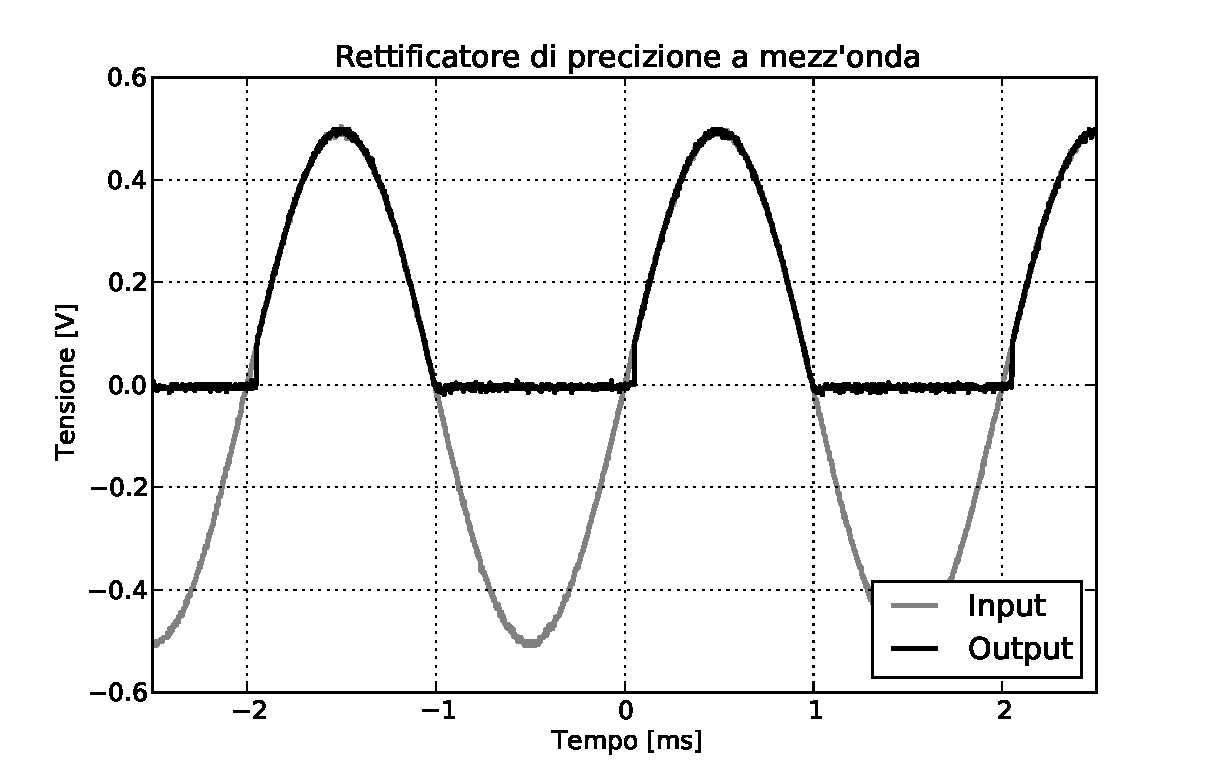
\includegraphics[width=0.7\textwidth]{figure/rett.pdf}
%        \caption{Questo grafico illustra l'andamento di $V\ped{out}$, linea nera, in funzione di $V\ped{in}$, linea grigia. Si nota chiaramente, come da previsioni, che la parte negativa del segnale in ingresso impediscse al diodo di condurre, pertanto la tensione di output risulta nulla. Inoltre, come si può osservare, il fronte di salita di $V\ped{out}$ presenta un leggero ritardo rispetto al segnale in ingresso $V\ped{in}$. Questo ritardo è stato stimato essere approssimativamente di circa $(152\pm10)\SI{}{\micro\second}$.}
%        \label{fig:radd_plot1}
%\end{SCfigure}
